\documentclass{beamer}

\usepackage{graphicx}
\usepackage{caption}

\mode<presentation>
{
  \usetheme{Warsaw}

  \setbeamercovered{transparent}
}

\title{Gradient Coding}

\author{Runtian Zhu \\ \texttt{zhurt23@m.fudan.edu.cn}}

\date{2023.10.7}

\begin{document}

\captionsetup[figure]{labelformat=empty}

\begin{frame}
  \titlepage
\end{frame}

% \begin{frame}{Outline}
%   \tableofcontents
% \end{frame}

\section{References}

\begin{frame}{References}

\begin{itemize}
    \item R. Tandon, Q. Lei, A. G. Dimakis, and N. Karampatziakis, “\textbf{Gradient coding: Avoiding stragglers in distributed learning},” in International Conference on Machine Learning, PMLR, 2017, pp. 3368–3376.
    \item L. Chen, H. Wang, Z. Charles, and D. Papailiopoulos, “\textbf{Draco: Byzantine-resilient distributed training via redundant gradients},” in International Conference on Machine Learning, PMLR, 2018, pp. 903–912.
    \item C. Hofmeister, L. Maßny, E. Yaakobi, and R. Bitar, “\textbf{Trading Communication for Computation in Byzantine-Resilient Gradient Coding},” arXiv preprint arXiv:2303.13231, 2023.
    
\end{itemize}

% \begin{figure}
%     \centering
%     \begin{minipage}[t]{.2\paperwidth}
%         \centering
%         
\includegraphics[width=\textwidth]{res/Rashish Tandon.jpg}
%         \caption{Rashish Tandon}
%     \end{minipage}
%     \begin{minipage}[t]{.2\paperwidth}
%         \centering
%         
\includegraphics[width=\textwidth]{res/Qi Lei.jpg}
%         \caption{Qi Lei}
%     \end{minipage}
%     \begin{minipage}[t]{.2\paperwidth}
%         \centering
%         
\includegraphics[width=\textwidth]{res/alexdimakis_sm.jpg}
%         \caption{Alexandros G. Dimakis}
%     \end{minipage}
%     \begin{minipage}[t]{.2\paperwidth}
%         \centering
%         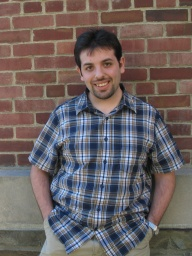
\includegraphics[width=\textwidth]{res/Nikos Karampatziakis.jpg}
%         \caption{Nikos Karampatziakis}
%     \end{minipage}
% \end{figure}

\end{frame}

\section{Gradient Coding}

\subsection{Background}

\begin{frame}{Distributed Learning}{Gradient Descent in Machine Learning}

\begin{block}{Gradient Descent}
    find $\boldsymbol{\theta}$ to minimize $L(\boldsymbol{\theta})$\ ($\boldsymbol{\theta}_0$ is chosen randomly):

    \[\boldsymbol{\theta}_{k + 1} = \boldsymbol{\theta}_{k} - \alpha\boldsymbol{\nabla} L(\boldsymbol{\theta})\]
\end{block}

\begin{block}{Loss Function}
    Suppose training set $D = \{(\boldsymbol{x}_1, \boldsymbol{y}_1), (\boldsymbol{x}_2, \boldsymbol{y}_2), (\boldsymbol{x}_m, \boldsymbol{y}_m)\}$. Let $\boldsymbol{X} = [\boldsymbol{x}_1, \boldsymbol{x}_2, \dots, \boldsymbol{x}_m]$, $\boldsymbol{Y} = [\boldsymbol{y}_1, \boldsymbol{y}_2, \dots, \boldsymbol{y}_m]$, $\boldsymbol{\theta}$ is hyperparameter, $l(\boldsymbol{\theta}, \boldsymbol{x}_i, \boldsymbol{y}_i)$ is the loss function. The total loss function is
    \[L(\boldsymbol{\theta}, \boldsymbol{X}, \boldsymbol{Y}) = \sum_{i}\frac{1}{m}l(\boldsymbol{\theta}, \boldsymbol{x}_i, \boldsymbol{y}_i)\]
\end{block}

\end{frame}

\begin{frame}{Distributed Learning}{Gradient Descent in Machine Learning}

\begin{block}{Gradient Descent}
    \[\boldsymbol{\theta}_{k + 1} = \boldsymbol{\theta}_{k} - \alpha\boldsymbol{\nabla} L(\boldsymbol{\theta})\]
\end{block}

\begin{block}{Loss Function}
    \[L(\boldsymbol{\theta}, \boldsymbol{X}, \boldsymbol{Y}) = \sum_{i}\frac{1}{m}l(\boldsymbol{\theta}, \boldsymbol{x}_i, \boldsymbol{y}_i)\]
\end{block}

\begin{block}{The linearity of gradient}
    \[\boldsymbol{\nabla} L(\boldsymbol{\theta}, \boldsymbol{X}, \boldsymbol{Y}) = \sum_{i}\boldsymbol{\nabla} \frac{1}{m}l(\boldsymbol{\theta}, \boldsymbol{x}_i, \boldsymbol{y}_i)\]
\end{block}

Gradient can be calculated distributedly!

\end{frame}

\begin{frame}{Distributed Learning}{Straggler Problem}

\begin{figure}
    \centering
    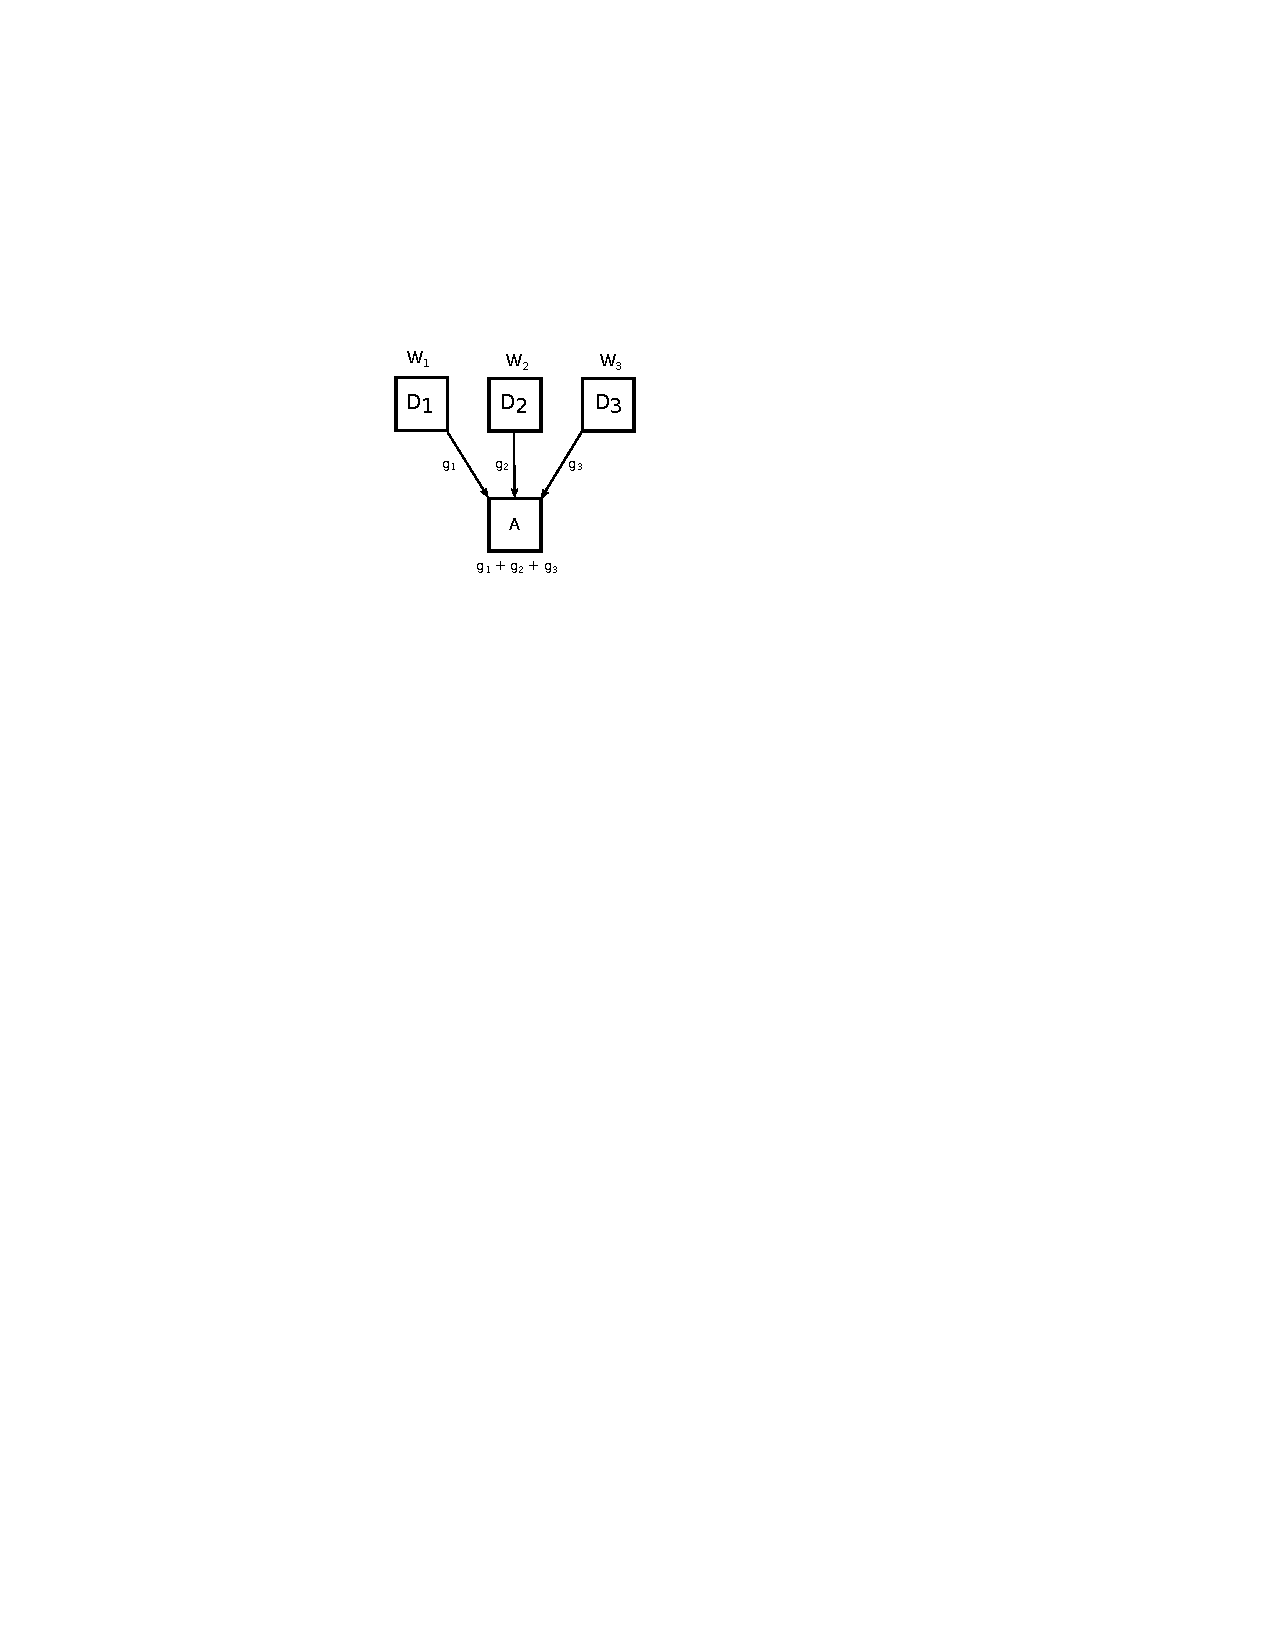
\includegraphics[height=.5\textheight]{res/distributed_learning.pdf}
\end{figure}

Problem:
\begin{itemize}
    \item Some workers may be stragglers (work much slower)
\end{itemize}

Possible Solutions:
\begin{itemize}
    \item Asynchronous SGD
    \item Synchronous minibatch SGD
\end{itemize}

\end{frame}

\subsection{An Example}

\begin{frame}{Distributed Learning}{Solution: replication}

\begin{figure}
    \centering
    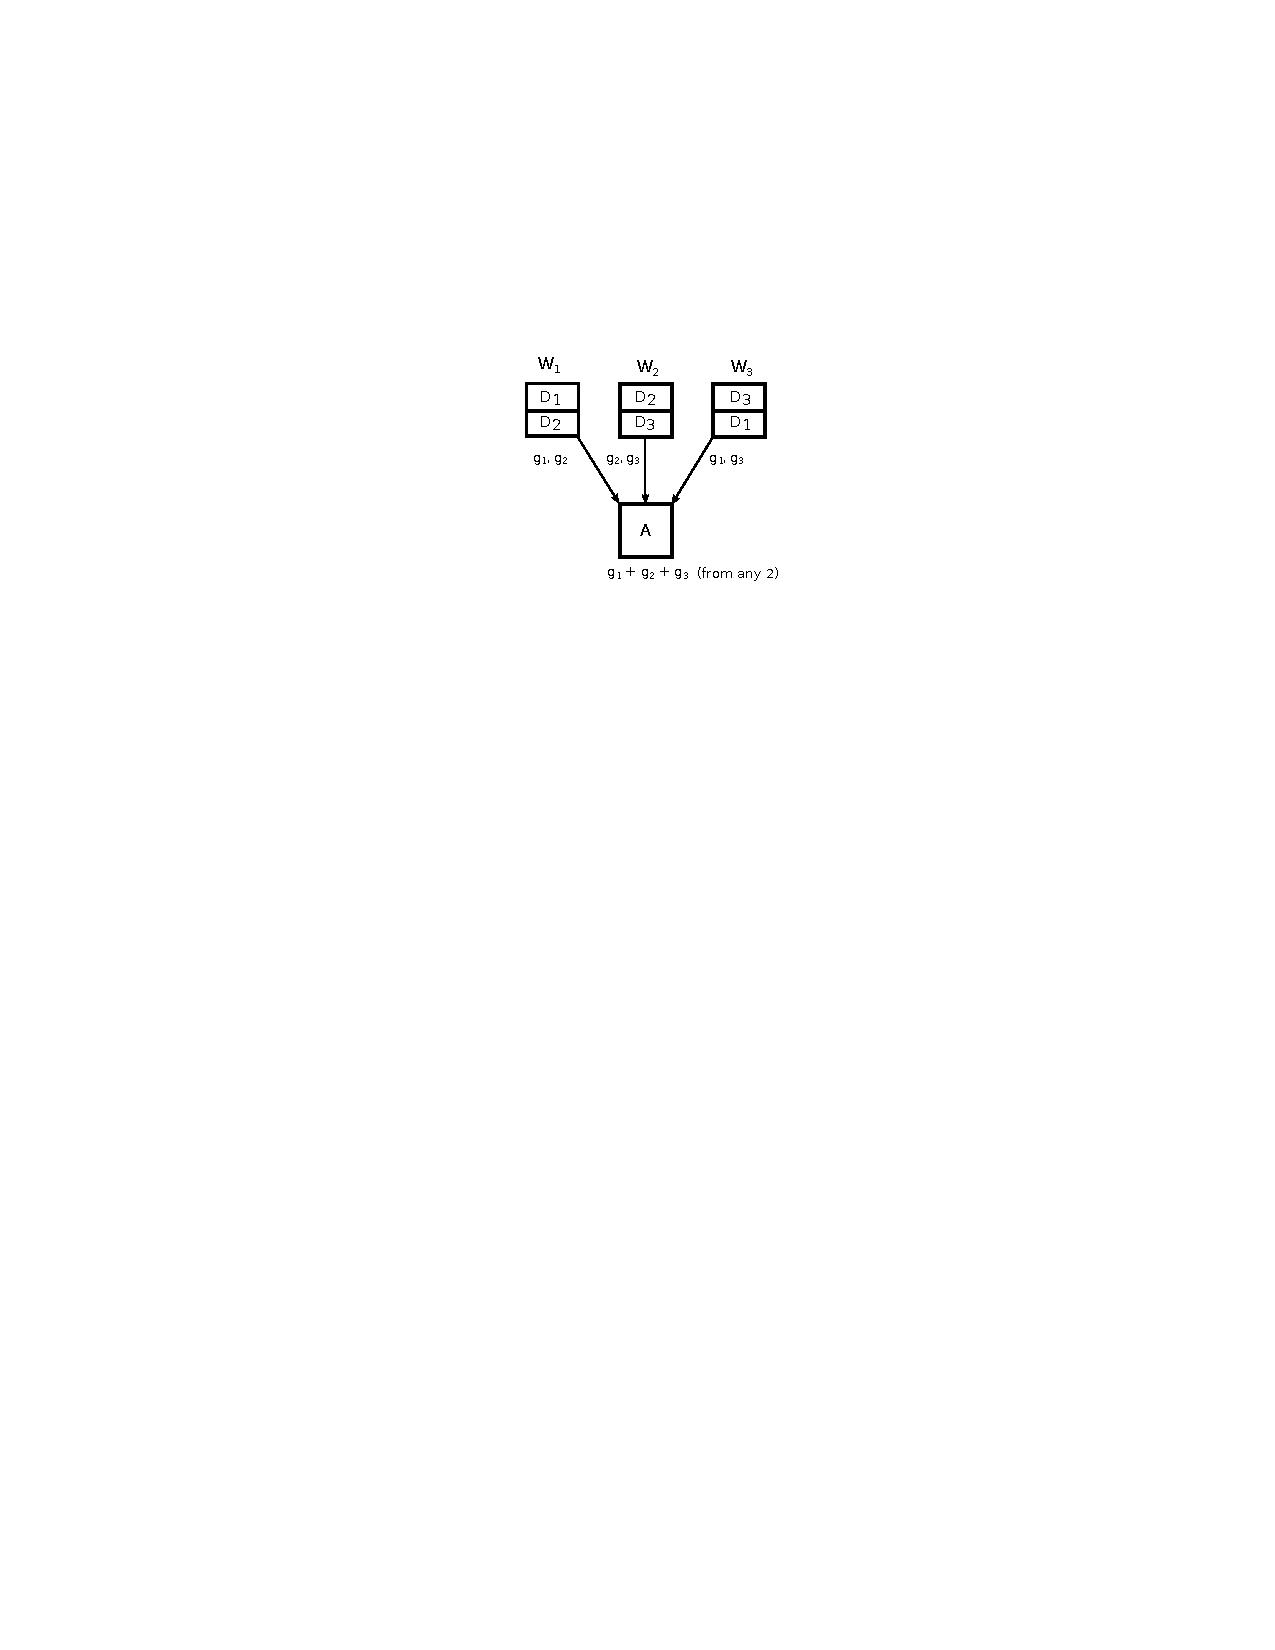
\includegraphics[height=.7\textheight]{res/replicate.pdf}
    % \begin{minipage}[t]{0.48\textwidth}
    %     \centering
    %     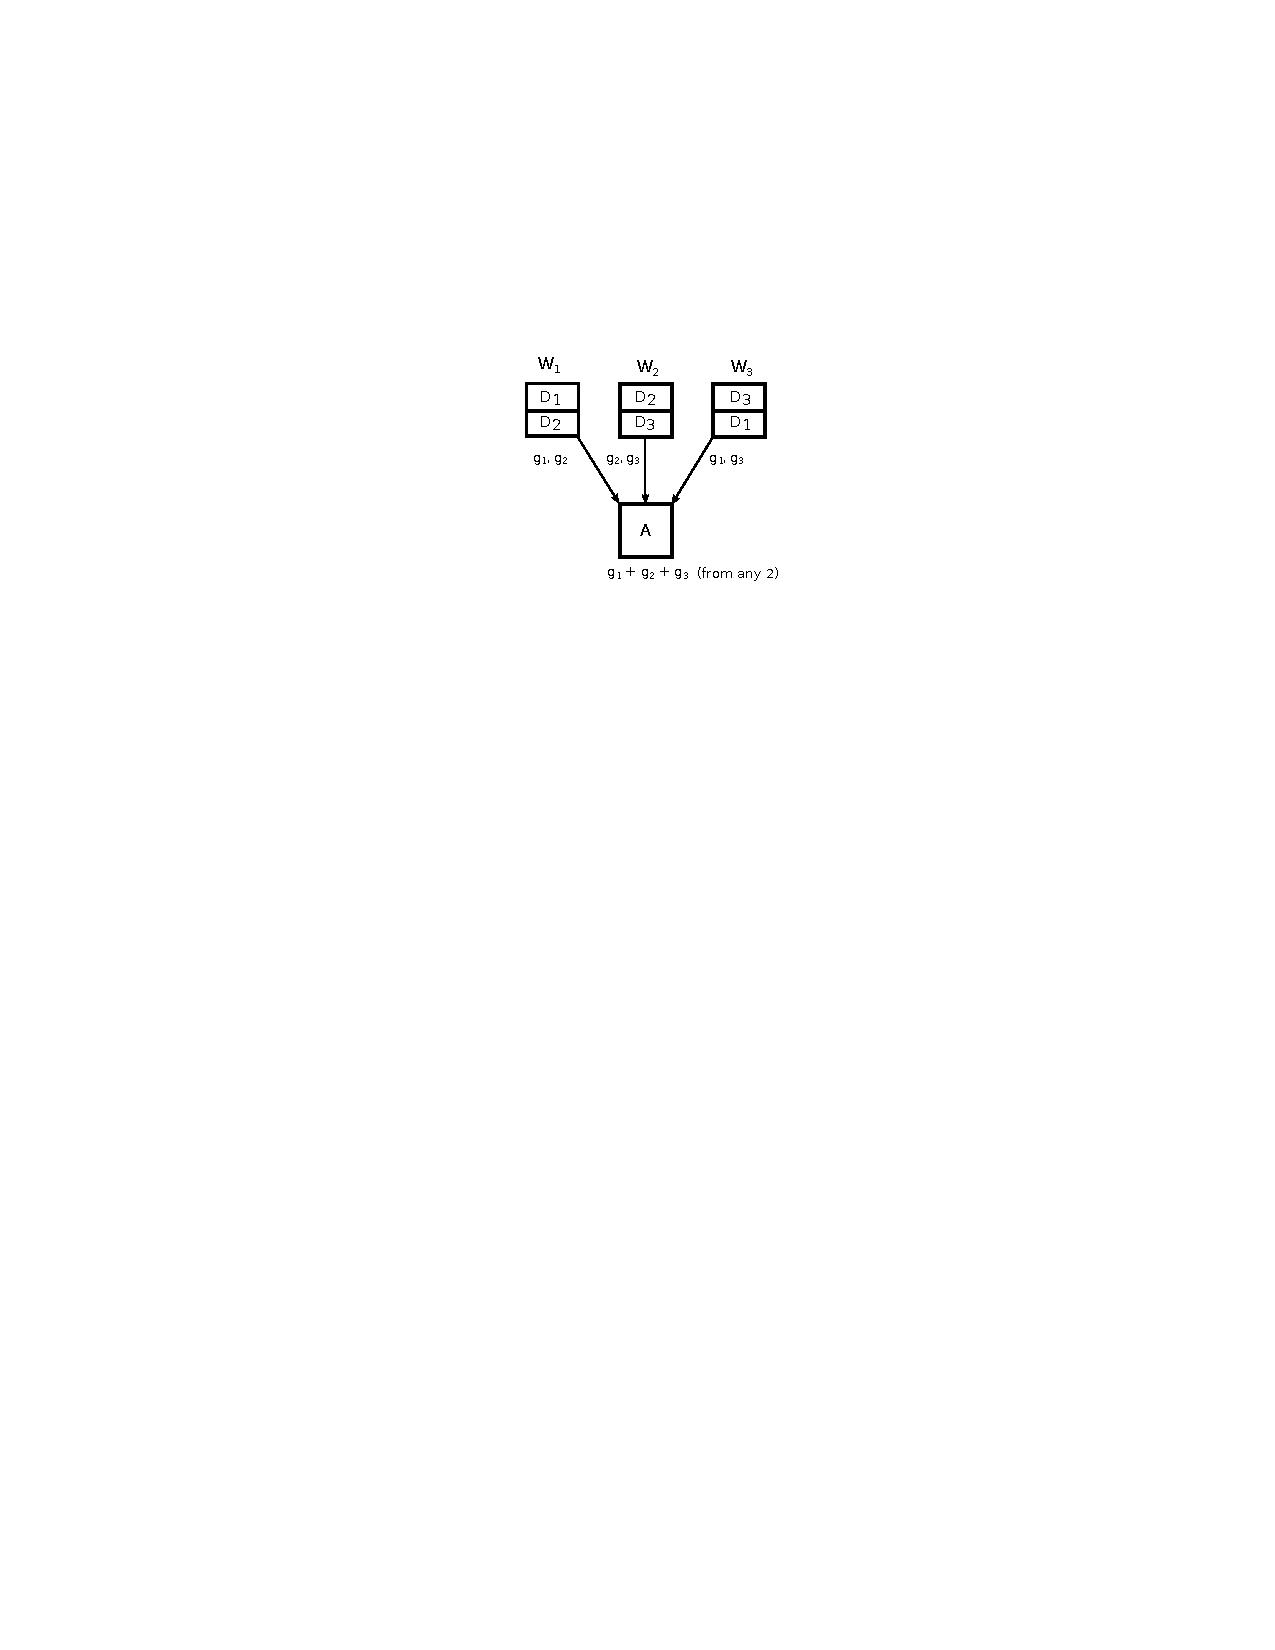
\includegraphics[width=\textwidth]{res/replicate.pdf}
    %     \caption{Replication}
    %     \end{minipage}
    %     \begin{minipage}[t]{0.48\textwidth}
    %     \centering
    %     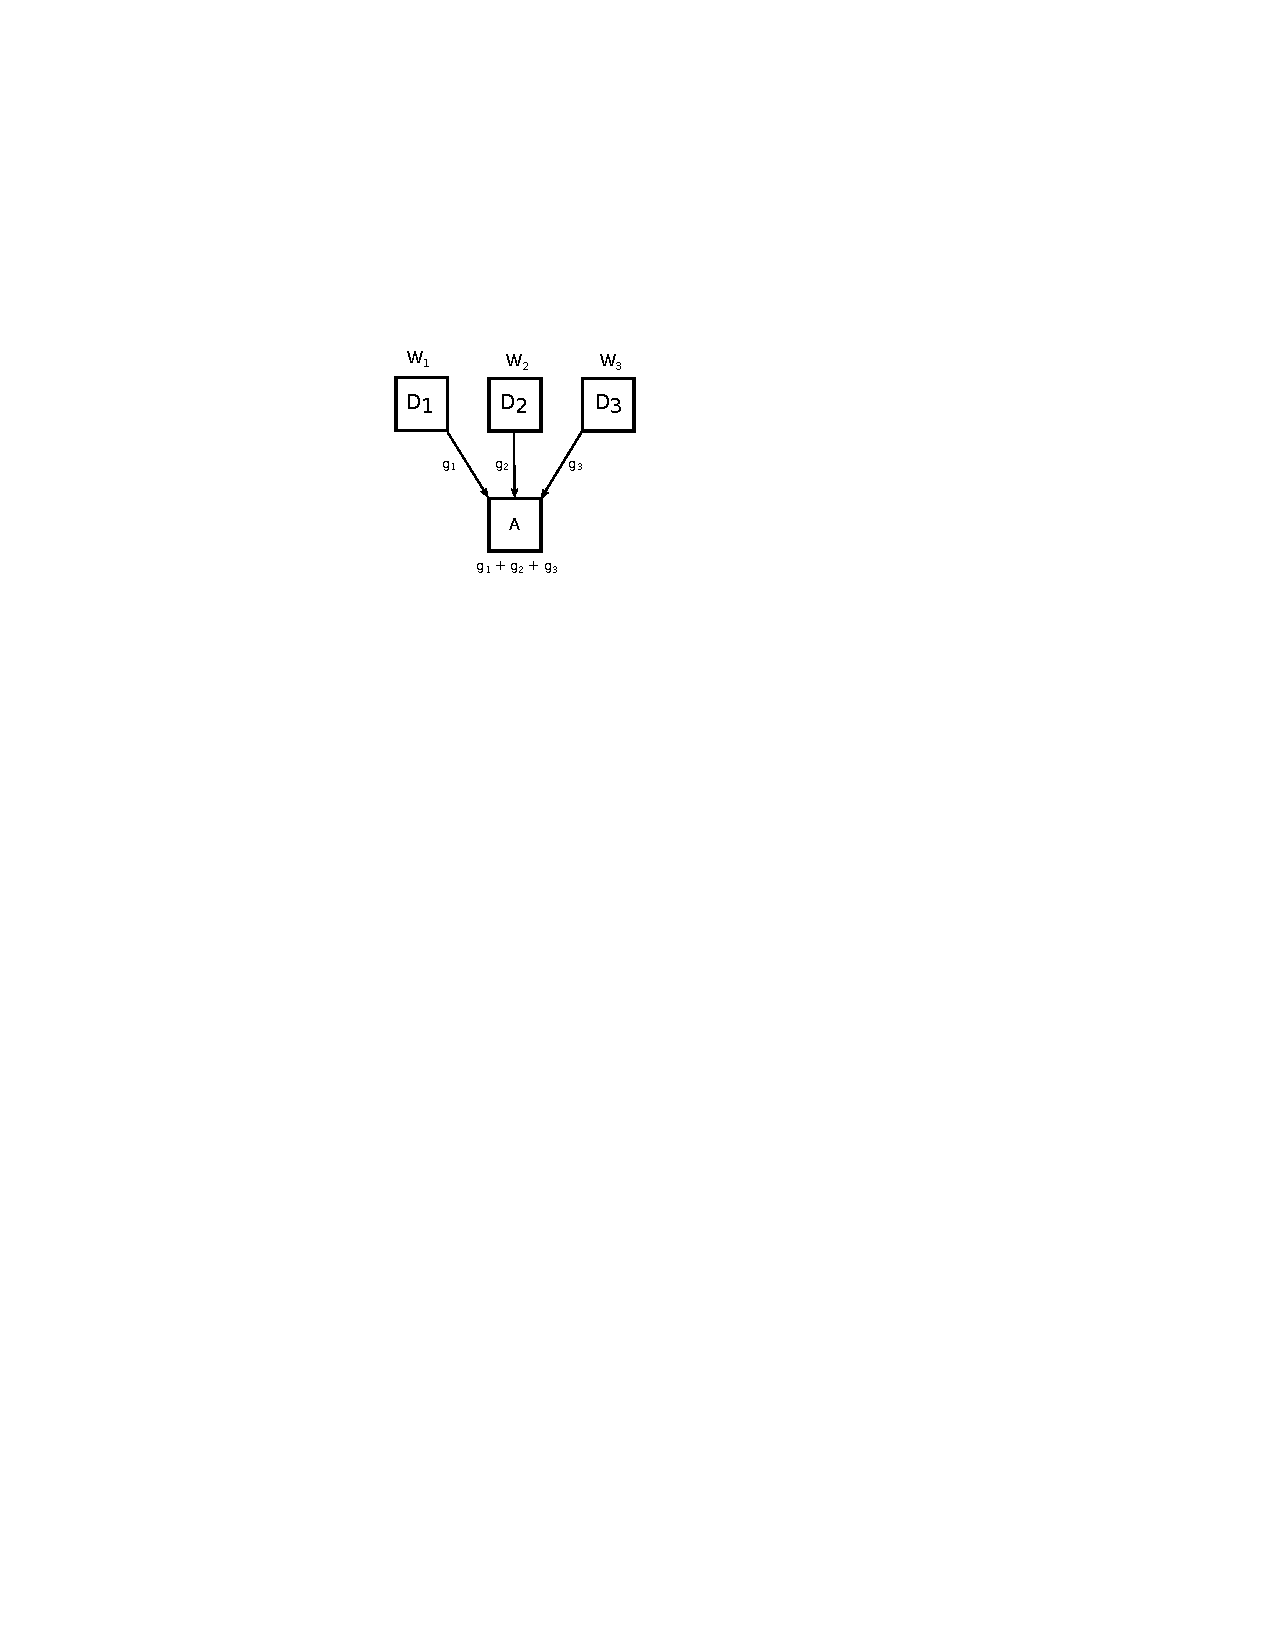
\includegraphics[width=\textwidth]{res/distributed_learning.pdf}
    %     \caption{Naive synchronous gradient descent}
    % \end{minipage}
\end{figure}

\end{frame}

\begin{frame}{Distributed Learning}{Gradient Coding}

\begin{figure}
    \centering
    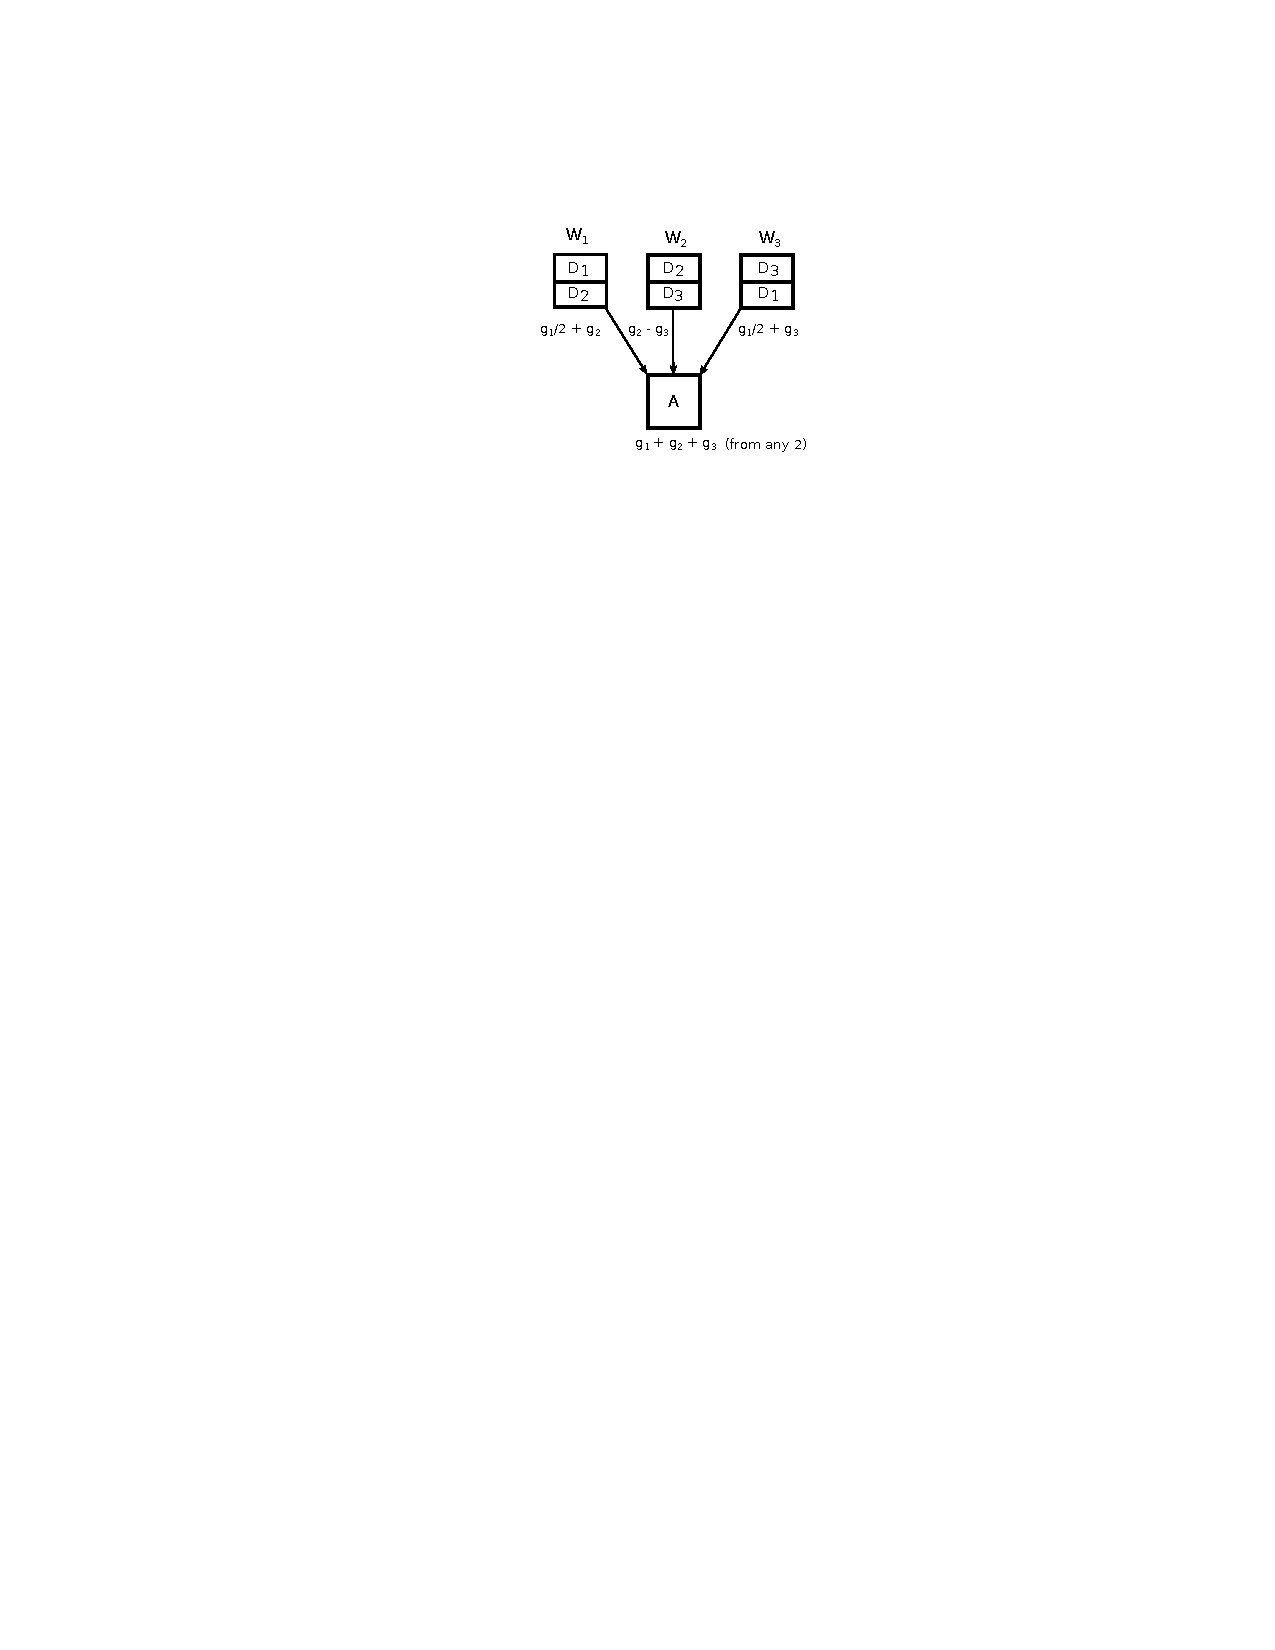
\includegraphics[height=.7\textheight]{res/gradient coding.pdf}
    % \begin{minipage}[t]{0.48\textwidth}
    %     \centering
    %     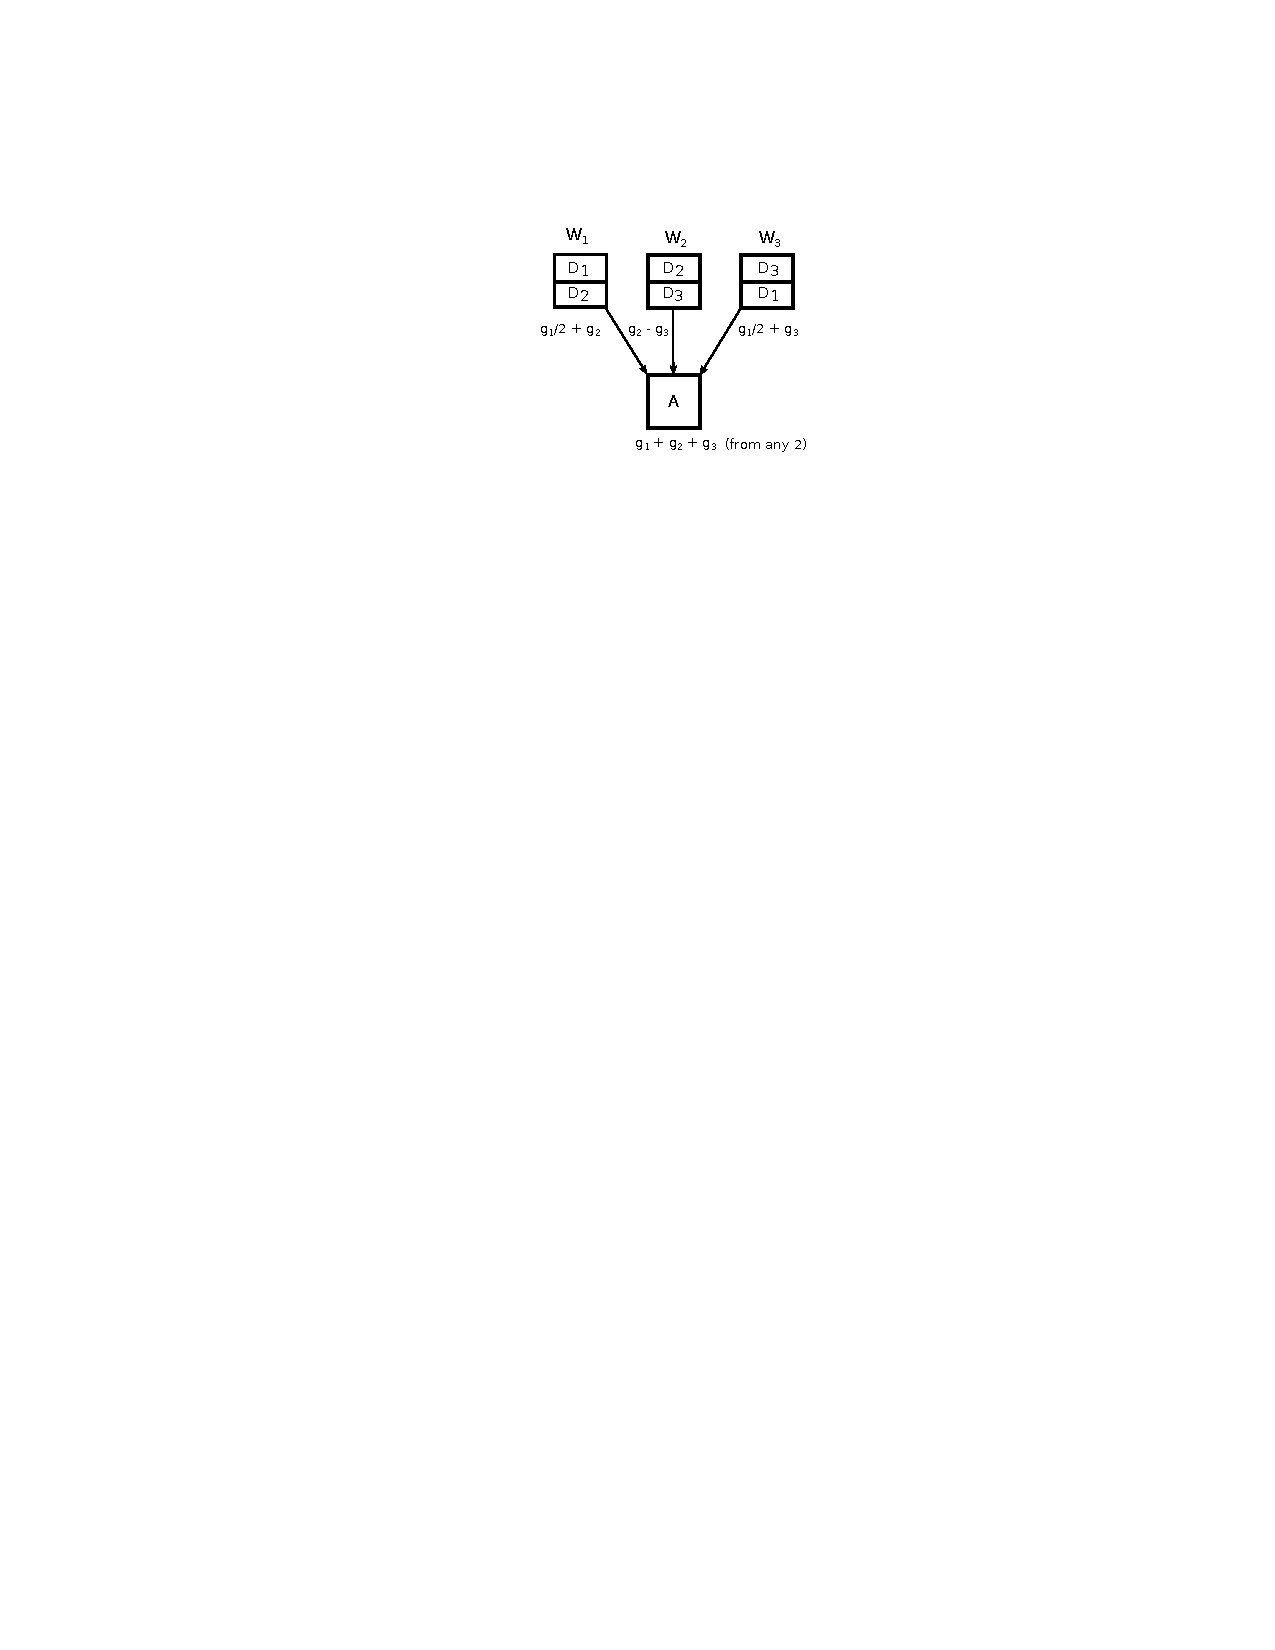
\includegraphics[width=\textwidth]{res/gradient coding.pdf}
    %     \caption{Gradient coding}
    %     \end{minipage}
    %     \begin{minipage}[t]{0.48\textwidth}
    %     \centering
    %     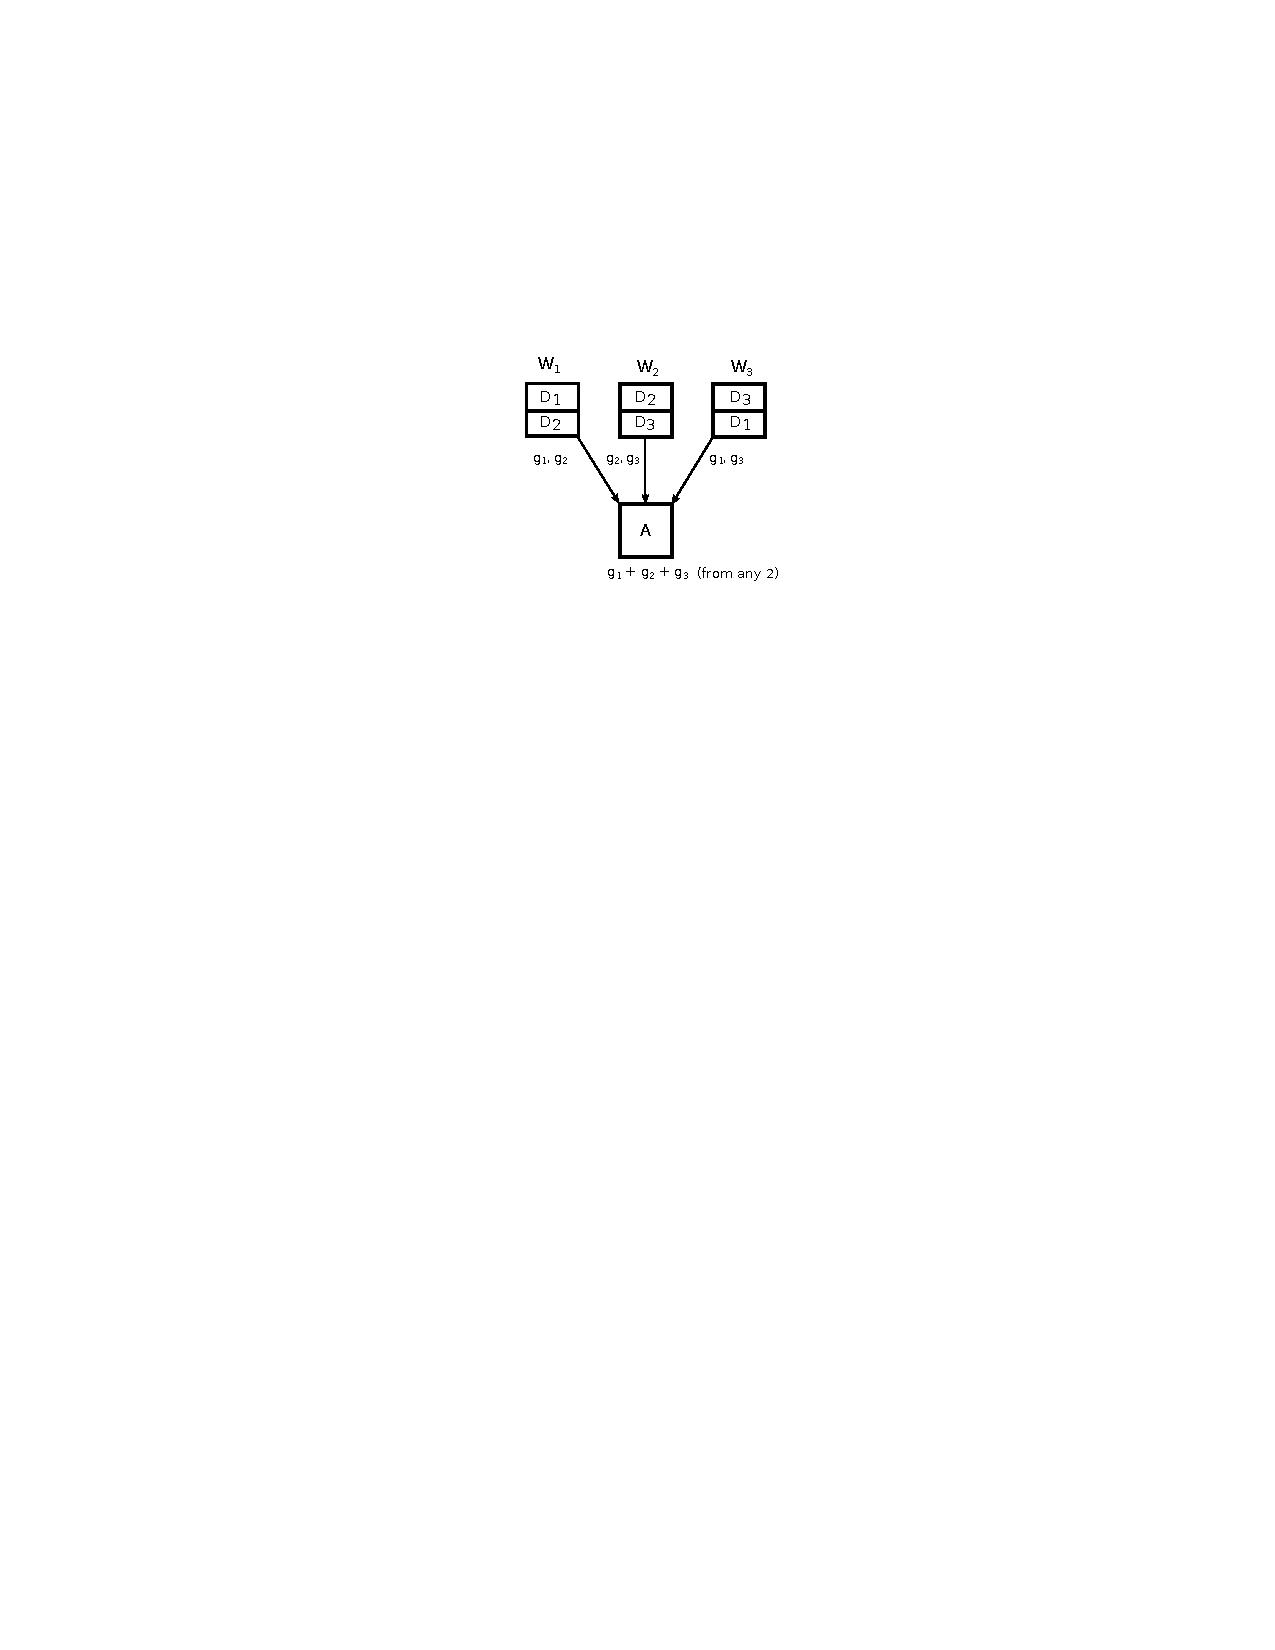
\includegraphics[width=\textwidth]{res/replicate.pdf}
    %     \caption{Replication}
    % \end{minipage}
\end{figure}

\end{frame}

\subsection{General Case}

\begin{frame}{Gradient Coding}{The General Setup}

\begin{definition}
    Let $f$ denotes the number of combinations of surviving workers/non-stragglers, $n$ denotes the number of workers, $k$ denotes the number of data partitions.
\end{definition}

\begin{definition}
    Let $A \in \mathbb{R}^{f \times n}$, the $i^{th}$ row of $A$ be $\boldsymbol{a_i}$. Each row of $A$ indicates a combination of surviving workers/non-stragglers.
\end{definition}

\begin{definition}
    Let $B \in \mathbb{R}^{n \times k}$, the $i^{th}$ row of $B$ be $\boldsymbol{b_i}$. $\boldsymbol{b_i}$ indicates the data partitions that the $i^{th}$ worker has access to.
\end{definition}

\end{frame}

\begin{frame}{Gradient Coding}{The General Setup}

\begin{block}{Conditions to be Met}
    \[AB = \boldsymbol{1}_{f\times k}\]
\end{block}

\begin{columns}

\begin{column}{.5\linewidth}
        
\begin{Example}
    \[A = \begin{bmatrix}
        0 & 1 & 2 \\
        1 & 0 & 1 \\
        2 & -1 & 0
    \end{bmatrix}\]
    
    \[B = \begin{bmatrix}
        1/2 & 1 & 0 \\
        0 & 1 & -1 \\
        1/2 & 0 & 1
    \end{bmatrix}\]
\end{Example}
    
\end{column}

\begin{column}{.5\linewidth}

\begin{figure}
    \centering
    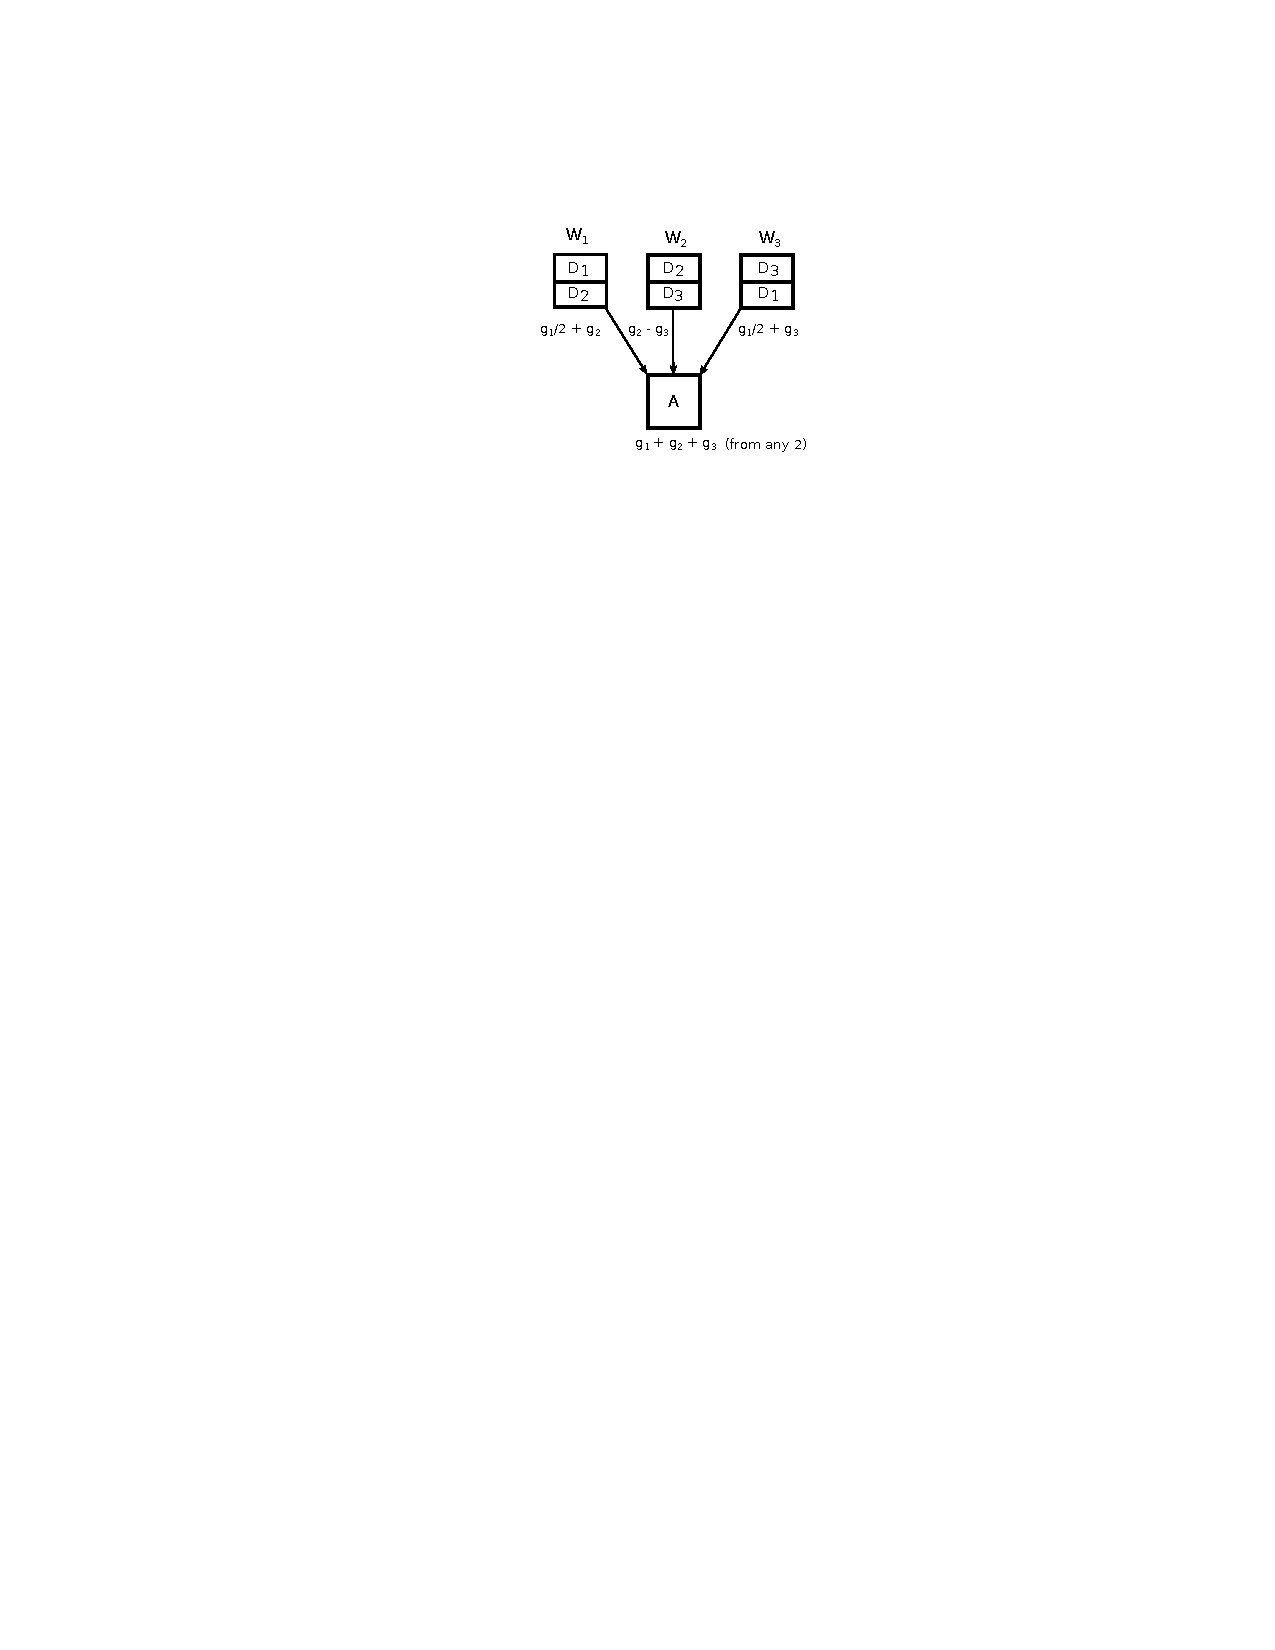
\includegraphics[width=\textwidth]{res/gradient coding.pdf}
\end{figure}

\end{column}

\end{columns}

\end{frame}

\begin{frame}{Gradient Coding}{The General Setup}

\begin{block}{Property}
    \[\boldsymbol{a_i}B\boldsymbol{\bar{g}} = \begin{bmatrix}
        1 & 1 & \dots & 1
    \end{bmatrix}\boldsymbol{\bar{g}} = (\sum_{j=1}^{k}\boldsymbol{g_j})^T\]
    \[\boldsymbol{a_i}B\boldsymbol{\bar{g}} = \sum_{k\in supp(\boldsymbol{a_i})}\boldsymbol{a_i}(j)(\boldsymbol{b_j} \boldsymbol{\bar{g}})\]
    where $\boldsymbol{\bar{g}} = \begin{bmatrix}
        \boldsymbol{g_1} & \boldsymbol{g_2} & \dots & \boldsymbol{g_k}
    \end{bmatrix}^T$, $\boldsymbol{g_i}$ denotes the gradient of the $i^{th}$ partition of work, $supp(\boldsymbol{x}) = \{i | x_i \neq 0\}$.
\end{block}


\end{frame}

\section{Further Work}

\subsection{DRACO}

\begin{frame}{DRACO}

\end{frame}

\subsection{Interactive Gradient Coding}

\begin{frame}{Interactive Gradient Coding}

\end{frame}

\end{document}

